\begin{refsection}
    \renewcommand{\thefigure}{\arabic{figure}}
    \renewcommand{\thetable}{\arabic{table}}
    
    \chapterTwoLines
    {Educação Ambiental nos livros de Geografia}
    {uma análise temática}
    \label{chap:educacao-ambiental-nos}

    \articleAuthor
    {Josemar Souza de Lima}
    {Graduado em Geografia pela Universidade Federal do Rio Grande do Norte (UFRN). Especialista em Educação Ambiental pelo Instituto de Educação Superior Presidente Kennedy (IFESP). Professor da rede pública estadual do RN. ID Lattes: 1537.5019.3163.5980. E-mail: josemar04souza@gmail.com.}
    
    \articleAuthor
    {Dayanne Chianca de Moura}
    {Professora Formadora do Instituto de Educação Superior Presidente Kennedy (IFESP). Doutora em Química pela Universidade Federal do Rio Grande do Norte (UFRN). ID Lattes: 5569.7390.4593.3136. ORCID: 0000-0002-5189-6332. E-mail: dayanne@ifesp.edu.br.}
    
    \begin{galoResumo}
        \marginpar{
            \begin{flushleft}
            \tiny \sffamily
            Como referenciar?\\\fullcite{SelfLimaAndMoura2021Educação}\mybibexclude{SelfLimaAndMoura2021Educação}, p. \pageref{chap:educacao-ambiental-nos}--\pageref{chap:educacao-ambiental-nosend}, \journalPubDate{}
            \end{flushleft}
        }
        Este artigo baseou-se no levantamento envolvendo uma amostragem de nove volumes de livros didáticos de geografia que eventualmente poderiam ser adotados pelas escolas públicas da rede estadual de ensino no Rio Grande do Norte --- triênio 2018--2020. O objetivo desse artigo foi fazer uma análise de quanto e como é abordado a temática e as questões ambientais nos mesmos. A pesquisa é de natureza aplicada, com abordagem qualitativa e quantitativa com objetivo exploratório. No que diz respeito aos procedimentos técnicos o trabalho é documental. A pesquisa, levantamento e análise dos dados coletados possibilitou verificar possíveis exageros, eficiências e ou deficiências, pôde apresentar um panorama das questões ambientais em uma disciplina que a priori está diretamente interligada com o meio ambiente em suas várias vertentes de estudo e discussões. Desta forma pôde-se verificar que os livros didáticos da ciência geográfica, de um modo geral, utilizados por nossos discentes, em nossa pesquisa, ficaram abaixo do que se poderia considerar eficiente e satisfatório na conexão, com as dimensões ambientais atuais, com seus desafios e avanços, no processo de ensino aprendizagem, visando a busca de proporcionar meios para a construção de uma sociedade mais crítica e consciente. 
    \end{galoResumo}
    
    \galoPalavrasChave{Educação. Livros. Temática Ambiental. Geografia.}

    \begin{otherlanguage}{english}

        \fakeChapterTwoLines
        {Environmental education in Geography textbooks}
        {a thematic analysis}
    
        \begin{galoResumo}[Abstract]
            This article was based on a survey involving a sample of nine volumes of geography textbooks that would eventually be adopted by public schools of the State of Rio Grande do Norte --- triennium 2018--2020. An analysis of how much and how it is approached the theme and the environmental issues in them. The research is applied in nature, with a qualitative and quantitative approach with an exploratory objective. As far as technical procedures are concerned, the work is documentary. The research, collection and analysis of the collected data allowed us to verify possible exaggerations, efficiencies and or deficiencies, that could show us a panorama of the environmental issues in a discipline that a priori is directly interconnected with the environment in its various aspects of study and discussions. In this way we could verify that the textbooks of geographic science, generally used by our students in our research, were below what we could consider efficient and satisfactory in connection with the current environmental dimensions with their challenges and advances, in the process of teaching learning, aiming the search to provide means for the construction of a more critical and conscious society. 
        \end{galoResumo}
        
        \galoPalavrasChave[Keywords]{Education. Books. Environmental Theme. Geography.}
    \end{otherlanguage}


    \section{Introdução}

    O processo educacional, tomando como um de seus principais pressupostos as práticas pedagógicas nas escolas é visto como um processo de grande importância para as urgentes transformações que a sociedade necessita, ou seja, uma sociedade mais justa, fraterna e ambientalmente sustentável. Desta forma, são muitos os pontos que permeiam a prática no cotidiano escolar, em que sobressai a urgência na aglutinação do que nós podemos chamar de dimensão ambiental, com ênfase no processo de ensino-aprendizagem, fator importante dessa prática.  

    Para isto, são muitos os elementos que interferem nessa aglutinação, como por exemplo, as políticas em educação ambiental, o nosso sistema educacional, a falta de recursos e investimentos em educação, o posicionamento docente, o interesse de discentes, a questão dos recursos educacionais, em especial o livro didático, entre outros  (MARPICA; LOGAREZZI, 2010).  

    Entre esses elementos, as políticas em educação são disposições que implicam todos os demais, repercutindo no resultado do ensino em geral. Destacam-se os Parâmetros Curriculares Nacionais (PCN) e a Política Nacional de Educação Ambiental (PNEA), instituída pela Lei 9.795/1999 \cite{PCN1999}, ambas propondo que a educação ambiental deva ter um caráter transversal na escola, não constituindo uma disciplina, mas permeando todas as já existentes (PCN, 1999). 

    A Base Nacional Comum Curricular \cite{BasNaCur2018} para a Educação Básica é um documento fruto de debate e negociação com diferentes atores do campo educacional e com a sociedade brasileira em geral, apresenta os Direitos e Objetivos de Aprendizagem e Desenvolvimento que devem orientar a elaboração de currículos para as diferentes etapas de escolarização na análise da amostragem dos nove volumes de livros didáticos de geografia do PNLD, triênio 2018--2020. 

    Com isso, podemos destacar a importância dessa pesquisa, uma vez que objetivou analisar critérios relacionados à abordagem da temática ambiental --- “Como (modo) e Quanto (frequência) é abordado a temática nos livros didáticos de geografia?”, a partir dos conteúdos, algo tão importante e previsto nos documentos orientadores da educação, além da educação ambiental e temas afins assegurados na Constituição Federal de 1988, art. 225 que assegura:  

    \begin{quotation}
        Todos têm direito ao meio ambiente ecologicamente equilibrado, bem de uso comum do povo e essencial à sadia qualidade de vida, impondo-se ao poder público e à coletividade o dever de defendê-lo e preservá-lo para as presentes e futuras gerações. \cite{ConstituiçãoBrasil1988}.
    \end{quotation}

    É importante ressaltar que o livro didático além de instrumento de apoio ao professor, é para o aluno uma valiosa ferramenta de pesquisa, consulta, estudo e contato com a cultura escrita, exercendo também, o relevante papel de formador de leitores, sendo em muitos lares um dos poucos suportes, que contêm gêneros textuais escritos, disponível para estudo ou desenvolvimento intelectual. Portanto, a sua escolha, pela equipe da escola, deve pautar-se na possibilidade e contribuição, que este objeto da cultura escolar possa promover para uma aprendizagem significativa.  

    Um bom livro de geografia e, em consonância com esse artigo, expõe a necessidade de observarmos e analisarmos como os volumes, alvo da nossa pesquisa, conduz a temática ambiental inserida nos temas e assuntos abordados. Neles podemos ter uma visão geral e crítica da temática ambiental, no que diz respeito a presença dela ou não no livro e ao modo como são abordados, para uma real contribuição na formação de cidadãos mais conscientes e preocupados com o futuro do nosso planeta, frente aos problemas ambientais a nível local, regional e global pelo qual estamos vivenciando cada vez mais, mediante os “avanços” da humanidade.  

    Nessa perspectiva, o livro didático de geografia, apresenta um papel de grande relevância, visto que está presente em sala de aula, auxiliando a implementação das políticas educacionais em geral e a abordagem da educação ambiental em âmbito formal, em que este dá um suporte no planejamento pedagógico de docentes. Desta forma, os livros didáticos da ciência geográfica associam há muito tempo o caráter transversal da educação ambiental que objetiva tratar essa temática considerada complexa na atualidade, principalmente sob a ótica de uma educação ambiental problematizadora, crítica e transformadora, ou seja, que encara a questão ambiental relacionada aos campos sociais, culturais e ideológicas, mencionados por tantos autores, como \textcite{CARVALHO2004Educação}, \textcite{LOUREIRO2006Problematizando}, \textcite{TOZONI-REIS2004Educação}, \textcite{SORRENTINO2005Educação}, Guimarães (2004) entre outros.  

    A amostragem utilizada para análise nesse trabalho foi selecionada com o objetivo de se verificar como a temática ambiental é trabalhada, se de forma gradativa, nos três volumes (1º, 2º e 3º anos) de cada uma das três coleções, resultando num total de nove volumes. Essa estratégia de escolha foi utilizada tendo em vista o universo total possuir vinte e sete volumes do triênio 2018--2020. Em seguida, ocorreu a análise de cada volume baseado nos critérios previamente definidos e estabelecidos. Concluída essa etapa, partiu-se para a organização dos dados e resultados, apresentados em tabelas e gráficos e posterior discussão dos resultados e considerações finais.  


    \section{O livro didático na educação básica brasileira}

    Nos últimos tempos, temos observado com o avanço do campo científico e da tecnologia que vários são os recursos disponíveis para auxiliar o docente em sua prática pedagógica. No entanto, o livro didático, ainda desempenha um relevante papel na educação em nosso país, uma vez que, muitos recursos didático-pedagógicos ainda não se encontram disponíveis em várias escolas por esse imenso país de dimensões continentais e de contrastes regionais. Desta forma, percebe-se a importância do melhoramento ou aprimoramento desse recurso que mesmo com o advento de outros materiais didáticos ainda poderá ser utilizado, uma vez que se for de boa qualidade e utilizado de forma correta é capaz de proporcionar resultados bastante positivos nos processos de ensino aprendizagem.  

    Sendo assim, propõe-se nesta abordagem, analisar o modelo teórico do livro didático de Geografia para o ensino básico, especificamente, do Ensino Médio. De acordo com \textcite{HESPANHOL2006Avaliação}:
    
    \begin{quotation}
        Um livro didático de Geografia deve primeiro, preparar o aluno para atuar num mundo complexo, localizar-se nele, decodificá-lo, compreender seu sentido e significado; e em seguida, desenvolver seu espírito crítico, que implica a capacidade de problematizar a realidade, propor soluções e reconhecer sua complexidade. \cite[p.~77]{HESPANHOL2006Avaliação}. 
    \end{quotation}

    Baseado nisto, percebe-se que um bom livro didático de Geografia além de apresentar informações e conceitos geográficos, deve, sobretudo, auxiliar tanto os docentes quanto os discentes na formulação de um raciocínio crítico, fundamentado em bases do conhecimento científico a fim de que esse recurso possa contribuir para estimular a criatividade dos envolvidos para que os mesmos possam entender e agir no mundo em que vivem de maneira que desenvolvam o respeito mútuo, tanto para com os seres humanos, como os demais seres vivos e os recursos naturais.  


    \section{Escolha do livro didático no brasil}

    Para escolha dos livros didáticos na avaliação pedagógica é importante o conhecimento do Guia do Programa Nacional do Livro Didático (PNLD). É tarefa de professores e equipe pedagógica analisar as resenhas contidas na guia para escolher adequadamente os livros a serem utilizados no triênio.  

    O livro didático deve ser adequado ao projeto político-pedagógico da escola; ao aluno e professor e a realidade sociocultural das instituições. Os professores podem selecionar os livros a serem utilizados em sala de aula somente pela internet, no portal do Fundo Nacional do Desenvolvimento da Educação (FNDE). A escola deve apresentar duas opções na escolha das obras para cada ano e disciplina. Caso não seja possível a compra da primeira opção, o FNDE envia à escola a segunda coleção escolhida. Portanto, a escolha da segunda opção deve ser tão criteriosa quanto a primeira.  

    No volume “Apresentação da Guia”, encontra-se as orientações referentes à escolha das coleções. O guia de livros didáticos é uma peça fundamental do PNLD e tem, a princípio, três funções: a primeira é orientar os docentes da Educação Básica para que possam melhor realizar o processo de escolha das obras que serão utilizadas no Brasil todo; a segunda função é facilitar o debate público e social a cerca dessa importante política pública, sendo mediador de concepções, afirmações e convocações com um impacto no campo do currículo e da experiência social; como terceira função, o guia apresenta os parâmetros de efetivação legal do Programa, contendo os elementos que norteiam os procedimentos de aquisição e distribuição das obras às escolas do País.  

    O PNLD é um programa consolidado como política de Estado, reconhecido por sua relevância nas escolas do país, devido às repercussões na qualidade dos processos de mediação pedagógica e à observância dos princípios éticos republicanos expressos em todas as fazes de sua execução, evidenciando o protagonismo docente e o compromisso com a melhoria da educação pública. 


    \section{Das obras para a análise: algumas informações gerais}

    As obras que fizeram parte da pesquisa e que foram aprovadas pelo PNLD 2018 são: \textit{Geografia: Espaço e Identidades} --- Levon Boligian e Andressa Alves, Editora do Brasil; \textit{Território e Sociedade no Mundo Globalizado} --- Elian Alibilluci, Anselmo Lazaro Branco e Cláudio Mendonça, Editora Saraiva; \textit{Fronteiras da Globalização} --- Lúcia Marina e Tércio, Editora Ática; \textit{Ser Protagonista} --- Flávio Manzato de Souza, Bianca Carvalho Vieira, Carla Bilheiro Santi, Carlos Henrique Jardim, Fernando dos Santos Sampaio e Ivone Siqueira Sucena (obra coletiva concebida, desenvolvida por Edições SM); \textit{Geografia: Ação e Transformações} --- Alice de Martini e Rogata Soares Del Gaudio, Editora Educacional; \textit{Geografia Geral e do Brasil: Espaço geográfico e globalizado} --- João Carlos Moreira e Eustáquio de Sene, Editora Scipione; \textit{Geografia das Redes: O mundo e seus lugares} --- Douglas Santos, Editora do Brasil; \textit{Geografia em rede} --- Edilson Adão e Laercio Furquim Jr., Editora FTD e; \textit{Geografia: Leituras e Interação} --- Arno Aloísio Gootens e Antonio Luís Joia, Editora Leya.


    \section{Metodologia}

    A presente pesquisa é de natureza aplicada, com abordagem qualitativa e quantitativa e com objetivo exploratório. No que diz respeito aos procedimentos técnicos o trabalho é documental.  

    A pesquisa realizada foi baseada na análise de livros didáticos do componente curricular de geografia que eventualmente podiam ser utilizados pelos alunos do ensino médio da rede estadual de ensino no estado do Rio Grande do Norte, no triênio de 2018 a 2020.  

    A presente pesquisa foi realizada a partir do levantamento e análise de nove volumes, escolhidos de forma aleatória, no universo de livros fornecidos pelas editoras envolvidas no processo de escolha dos livros didáticos, para a disciplina de geografia, junto à Secretaria de Educação do Estado do Rio Grande do Norte e ao Programa Nacional do Livro Didático (PNLD), em que os professores das instituições de ensino deliberam sobre a escolha deles.  

    Para o desenvolvimento deste trabalho foi feito o levantamento, observação e a posterior análise com ênfase na verificação da temática ambiental em cada volume, em consonância com o objetivo deste trabalho. A definição das categorias e critérios para a análise dos livros didáticos fundamentou-se em aspectos teórico-metodológicos, aspectos pedagógico-metodológicos e aspectos visuais. Os critérios foram determinados com base em livros e artigos ligados à temática dos livros didáticos \cite{BANDEIRAAndSTANGEAndSANTOS2012Proposta}. Para a materialização dos procedimentos elaboramos tabelas e gráficos que serão apresentados posteriormente.


    \section{Análise dos livros didáticos}

    Quanto aos critérios para análise das coleções, optou-se por observar a frequência e modo como a temática e as questões ambientais são abordados nos volumes alvo dessa pesquisa. Quando da construção e escolha da temática para o desenvolvimento dessa pesquisa, foram escolhidas como objeto de investigação a observação e análise de livros didáticos de geografia e, no que diz respeito à abordagem e sua frequência da temática ambiental.  

    Inicialmente foi pensado em analisar todas as coleções contempladas e disponibilizadas nas escolas para escolha dos professores da disciplina de geografia. Foram aprovadas no PNLD 2018--2020 nove coleções, perfazendo o total de vinte e sete volumes. A partir dessa constatação, isto é, um universo um tanto abrangente e considerando os anseios norteadores desse trabalho, foram escolhidas três coleções. Cada uma inclui os livros do 1º, 2º e 3º anos totalizando uma amostragem de nove volumes, ao qual codificamos de L1A, L1B, L1C, L2A, L2B, L2C, L3A, L3B e L3C, garantindo assim uma amostragem de 33\% das obras previstas no PNLD para a disciplina de geografia.  

    Depois de selecionados os volumes a serem analisados, foi construído um roteiro para a análise dos livros, trazendo inicialmente um breve resumo relacionando a abrangência do ensino de geografia no ensino médio, com a escolha do livro didático nesta etapa de ensino, destacando a importância das questões ambientais neste componente curricular.  

    A Tabela \ref{tble:relacao-livros} apresenta as características gerais de todos os nove volumes analisados e avaliados.

    \begin{table}
        \centering

        \caption{Relação das coleções dos livros didáticos de Geografia para a avaliação para o triênio 2018--2020, do Programa do Livro Didático (PNLD)}
        \label{tble:relacao-livros}

        \makebox[\textwidth]{\begin{tabular}[!ht]{
            >{\small}c
            >{\small}c
            >{\small}c
            >{\small}c
            >{\small}c
            >{\small}c
            >{\small}c
        }
            \toprule
            Coleção & Livro & Autor & Editora & Edição & Ano & Código \\
            \midrule
            
            %% first row
            Leituras e interação & Geografia 1 & A. A. Gootens & \multirow{2}{*}{Leya} & \multirow{2}{*}{2ª} & \multirow{2}{*}{2016} & \multirow{2}{*}{0117P18053} \\
            (L1A) & (Ens. Médio) & A. L. Joia & & & & \\ [1ex]


            %% second row
            & & B. C. d. Souza & & & & \\
            & & Carla B. Santi & & & & \\
            Ser protagonista & Geografia 1 & Carlos B. Santi & \multirow{2}{*}{SM} & \multirow{2}{*}{3ª} & \multirow{2}{*}{2016} & \multirow{2}{*}{0075P18053} \\
            (L1B) & (Ens. Médio) & C. H. Jardim & & & & \\
            & & F. d. S. Sampaio & & & & \\
            & & I. S. Sucena & & & & \\ [1ex]

            %% third row
            Ação e transformação & Geografia 1 & A. d. Martini & \multirow{2}{*}{Escala} & \multirow{2}{*}{1ª} & \multirow{2}{*}{2016} & \multirow{2}{*}{0123P18053} \\
            (L1C) & (Ens. Médio) & R. S. d. Gaudio & & & & \\ [1ex]

            %% fourth row
            Fronteiras da globali-& & & & & & \\
            zação: o espaço geo-& Ensino Médio & \multirow{2}{*}{L. M. e Tércio} & \multirow{2}{*}{Ática} & \multirow{2}{*}{3ª} & \multirow{2}{*}{2017} & \multirow{2}{*}{0026P18053} \\
            gráfico globalizado& (2º ano) & & & & & \\
            (L2A) & & & & & & \\ [1ex]

            %% fifth row
            Geografia das redes: o & \multirow[b]{1.5}{*}{Geografia} & & & & & \\
            mundo e seus lugares & & D. Santos & Brasil & 3ª & 2016 & 0186P18053 \\
            (L2B) & \multirow[t]{-1.5}{*}{(Ens. Médio 2)} & & & & & \\ [1ex]

            %% sixth row
            Geografia: espaço e & \multirow[b]{1.5}{*}{Geografia 2} & \multirow[b]{1.5}{*}{L. Boligion} & & & & \\
            identidade & & & Brasil & 1ª & 2017 & 0174P18053 \\
            (L2C) & \multirow[t]{-1.5}{*}{(Ens. Médio)} & \multirow[t]{-1.5}{*}{A. Alves} & & & & \\ [1ex]

            %% seventh row
            Geografia geral e do & & & & & \\
            Brasil: espaço geográ- & Geografia 3 & J. C. Moreira & \multirow{2}{*}{Scipione} & \multirow{2}{*}{3ª} & \multirow{2}{*}{2017} & \multirow{2}{*}{0046P18053} \\
            fico e globalização & (Ens. Médio) & E. d. Sene & & & & \\
            (L3A) & & & & & & \\ [1ex]

            %% eighth row
            Território e sociedade & \multirow[b]{1.5}{*}{Geografia 3} & E. A. Lucci & & & & \\
            no mundo globalizado & & A. L. Branco & Saraiva & 3ª & 2017 & 0103P18053 \\
            (L3B) & \multirow[t]{-1.5}{*}{(Ens. Médio)} & C. Mendonça & & & & \\ [1ex]

            %% ninth row
            Geografia em rede & Geografia 3 & E. Adão & \multirow{2}{*}{FTD} & \multirow{2}{*}{2ª} & \multirow{2}{*}{2016} & \multirow{2}{*}{0132P18053} \\
            (L3C) & (Ens. Médio) & L. Furquin Jr. & & & & \\

            \bottomrule
        \end{tabular}}
        \caption*{Fonte: Guia de Livros Didáticos}
    \end{table}


    \section{Resultados e discussão}

    O ensino de Geografia, no Ensino Médio, expressa uma continuidade e ênfase às unidades desenvolvidas nos anos finais do Ensino Fundamental, como também dos anos iniciais, direcionando para estudos posteriores, isso de maneira mais crítica e questionadora, tratando de novos conhecimentos, em níveis de aprofundamento e de complexidades maiores. Nessa fase do Ensino Médio, os questionamentos e novas realidades apresentadas aos alunos, e as que eles mesmos observam e constroem, são sem dúvida mais complexas, tornando os anseios e os desafios vivenciados por eles bem mais abrangentes e desafiadores. Desta forma, se evidencia e se torna extremamente necessário a escolha do livro didático que possibilite aos alunos da disciplina de Geografia o desenvolvimento e a percepção de um olhar cada vez mais crítico e questionador da realidade que os cerca.  

    Baseado nisto, percebemos a educação ambiental como área de conhecimento pertencente no âmbito escolar como ferramenta transformadora no meio social, com isso, julgamos que a disciplina de Geografia tem profunda relação com as questões ambientais, demonstrando que o livro didático desta disciplina tem uma significativa contribuição no processo de ensino-aprendizagem, que envolve docentes e discentes. Seguindo a estrutura organizacional da Base Nacional Comum Curricular (BNCC/2018) para a Educação Básica. 

    A Tabela \ref{tble:classificacao-livros} apresenta as categorias e critérios e os conceitos Fraco (F), Bom (B), Ótimo (O), Excelente (E) para a análise das coleções dos livros didáticos de geografia para a avaliação, triênio 2018--2020, do PNLD.  

    Nesta tabela, foram considerados dois importantes critérios que segundo nossa avaliação contempla a problemática dessa pesquisa que é a ``Relevância na ocorrência da temática ambiental'' e ``Como a temática e as questões ambientais são abordadas''.

    \begin{table}
        \centering

        \caption{Análise das coleções de livros didáticos de Geografia para a avaliação para o triênio 2018--2020, do Programa do Livro Didático (PNLD) por critérios e categorias}
        \label{tble:classificacao-livros}

        \makebox[\textwidth]{\begin{tabular}[!ht]{
            >{\small}l
            >{\small}l
            >{\small}c
            >{\small}c
            >{\small}c
            >{\small}c
            >{\small}c
            >{\small}c
            >{\small}c
            >{\small}c
            >{\small}c
        }
            \toprule
            \multirow{2}{*}{ } & \multirow{2}{*}{Critérios} & \multicolumn{9}{c}{Livros} \\
            & & L1A & L1B & L1C & L2A & L2B & L2C & L3A & L3B & L3C \\
            \midrule

            % 1st row [2]
            \multirow{21}{*}{\rotatebox[origin=c]{90}{CONTEÚDOS}} & \multirow{2}{*}{Clareza conceitual} & \multirow{2}{*}{O} & \multirow{2}{*}{O} & \multirow{2}{*}{O} & \multirow{2}{*}{O} & \multirow{2}{*}{B} & \multirow{2}{*}{O} & \multirow{2}{*}{O} & \multirow{2}{*}{O} & \multirow{2}{*}{O} \\ 
            & & & & & & & & \\ [1ex]

            % 2nd row [2]
            & Adequação ao nível de & \multirow{2}{*}{O} & \multirow{2}{*}{O} & \multirow{2}{*}{O} & \multirow{2}{*}{O} & \multirow{2}{*}{O} & \multirow{2}{*}{O} & \multirow{2}{*}{O} & \multirow{2}{*}{O} & \multirow{2}{*}{O} \\
            & maturidade do aluno & & & & & & & \\ [1ex]

            % 3rd row [2]
            & Considerações às ideias & \multirow{2}{*}{O} & \multirow{2}{*}{O} & \multirow{2}{*}{O} & \multirow{2}{*}{O} & \multirow{2}{*}{O} & \multirow{2}{*}{O} & \multirow{2}{*}{O} & \multirow{2}{*}{O} & \multirow{2}{*}{O} \\
            & prévias dos alunos & & & & & & & \\ [1ex]

            % 4th row [2]
            & \multirow{2}{*}{Relações interdisciplinares} & \multirow{2}{*}{B} & \multirow{2}{*}{O} & \multirow{2}{*}{B} & \multirow{2}{*}{B} & \multirow{2}{*}{F} & \multirow{2}{*}{O} & \multirow{2}{*}{O} & \multirow{2}{*}{O} & \multirow{2}{*}{B} \\
            & & & & & & & & \\ [1ex]

            % 5th row [2]
            & Contextualização dos & \multirow{2}{*}{O} & \multirow{2}{*}{O} & \multirow{2}{*}{O} & \multirow{2}{*}{B} & \multirow{2}{*}{B} & \multirow{2}{*}{O} & \multirow{2}{*}{O} & \multirow{2}{*}{O} & \multirow{2}{*}{O} \\
            & assuntos & & & & & & & \\ [1ex]

            % 6th row [2]
            & Leituras complementares & \multirow{2}{*}{O} & \multirow{2}{*}{O} & \multirow{2}{*}{O} & \multirow{2}{*}{F} & \multirow{2}{*}{B} & \multirow{2}{*}{O} & \multirow{2}{*}{O} & \multirow{2}{*}{O} & \multirow{2}{*}{O} \\
            & disponíveis & & & & & & & \\ [1ex]

            % 7th row [2]
            & \multirow{2}{*}{Linguagem conceitual} & \multirow{2}{*}{O} & \multirow{2}{*}{O} & \multirow{2}{*}{O} & \multirow{2}{*}{B} & \multirow{2}{*}{B} & \multirow{2}{*}{O} & \multirow{2}{*}{O} & \multirow{2}{*}{O} & \multirow{2}{*}{O} \\
            & & & & & & & & \\ [1ex]

            % 8th row [2]
            & Relevância na ocorrência & \multirow{2}{*}{O} & \multirow{2}{*}{F} & \multirow{2}{*}{O} & \multirow{2}{*}{F} & \multirow{2}{*}{F} & \multirow{2}{*}{F} & \multirow{2}{*}{F} & \multirow{2}{*}{B} & \multirow{2}{*}{F} \\
            & da temática ambiental & & & & & & & \\ [1ex]

            % 9th row [2]
            & Como é abordada a temática & \multirow{2}{*}{O} & \multirow{2}{*}{F} & \multirow{2}{*}{O} & \multirow{2}{*}{F} & \multirow{2}{*}{F} & \multirow{2}{*}{F} & \multirow{2}{*}{F} & \multirow{2}{*}{B} & \multirow{2}{*}{F} \\
            & e as questões ambientais & & & & & & & \\

            \midrule

            % 1st row [2]
            \multirow{6.65}{*}{\rotatebox[origin=c]{90}{RECURSOS VISUAIS}} & Apresentação de objetos & \multirow{2}{*}{O} & \multirow{2}{*}{O} & \multirow{2}{*}{O} & \multirow{2}{*}{O} & \multirow{2}{*}{B} & \multirow{2}{*}{O} & \multirow{2}{*}{O} & \multirow{2}{*}{O} & \multirow{2}{*}{O} \\ 
            & gráficos e tabelas & & & & & & & \\ [1ex]

            % 2nd row [2]
            & Qualidade gráfica das & \multirow{2}{*}{O} & \multirow{2}{*}{O} & \multirow{2}{*}{O} & \multirow{2}{*}{O} & \multirow{2}{*}{O} & \multirow{2}{*}{O} & \multirow{2}{*}{O} & \multirow{2}{*}{O} & \multirow{2}{*}{O} \\
            & imagens & & & & & & & \\ [1ex]

            % 3rd row [2]
            & Coerência científica das & \multirow{2}{*}{O} & \multirow{2}{*}{O} & \multirow{2}{*}{O} & \multirow{2}{*}{O} & \multirow{2}{*}{O} & \multirow{2}{*}{O} & \multirow{2}{*}{O} & \multirow{2}{*}{O} & \multirow{2}{*}{O} \\
            & imagens & & & & & & & \\

            \midrule

            % 1st row [2]
            \multirow{6.65}{*}{\rotatebox[origin=c]{90}{ATIVIDADES}} & Proposição de problematização & \multirow{2}{*}{O} & \multirow{2}{*}{O} & \multirow{2}{*}{O} & \multirow{2}{*}{B} & \multirow{2}{*}{B} & \multirow{2}{*}{O} & \multirow{2}{*}{O} & \multirow{2}{*}{O} & \multirow{2}{*}{O} \\ 
            & nas atividades & & & & & & & \\ [1ex]

            % 2nd row [2]
            & Apresentação de conexão com & \multirow{2}{*}{O} & \multirow{2}{*}{O} & \multirow{2}{*}{O} & \multirow{2}{*}{B} & \multirow{2}{*}{B} & \multirow{2}{*}{O} & \multirow{2}{*}{O} & \multirow{2}{*}{O} & \multirow{2}{*}{O} \\
            & o cotidiano & & & & & & & \\ [1ex]

            % 3rd row [2]
            & Sistematização do conhecimento & \multirow{2}{*}{O} & \multirow{2}{*}{O} & \multirow{2}{*}{O} & \multirow{2}{*}{O} & \multirow{2}{*}{B} & \multirow{2}{*}{O} & \multirow{2}{*}{O} & \multirow{2}{*}{O} & \multirow{2}{*}{O} \\
            & através de exercícios diversos & & & & & & & \\

            \bottomrule
            & \multicolumn{8}{l}{\footnotesize \textsf{Legenda: Fraco (F), Bom (B), Ótimo(O), Excelente (E)}} & 
            \multicolumn{2}{r}{\footnotesize \textsf{\textit{continua}}}\\
        \end{tabular}}
    \end{table}

    \begin{table}
        \caption*{Tabela \ref{tble:classificacao-livros}~--~\textit{continuação da página anterior}}

        \makebox[\textwidth]{\begin{tabular}[!ht]{
            >{\small}l
            >{\small}l
            >{\small}c
            >{\small}c
            >{\small}c
            >{\small}c
            >{\small}c
            >{\small}c
            >{\small}c
            >{\small}c
            >{\small}c
        }

        \toprule
        \multirow{2}{*}{ } & \multirow{2}{*}{Critérios} & \multicolumn{9}{c}{Livros} \\
        & & L1A & L1B & L1C & L2A & L2B & L2C & L3A & L3B & L3C \\
        \midrule

        % 1st row [2]
        \multirow{6.5}{*}{\rotatebox[origin=c]{90}{PESQUISA}} & Apresentação de fontes para & \multirow{2}{*}{O} & \multirow{2}{*}{O} & \multirow{2}{*}{O} & \multirow{2}{*}{B} & \multirow{2}{*}{B} & \multirow{2}{*}{O} & \multirow{2}{*}{O} & \multirow{2}{*}{O} & \multirow{2}{*}{O} \\ 
        & consulta no livro & & & & & & & \\ [1ex]

        % 2nd row [2]
        & Incentivo à pesquisa & \multirow{2}{*}{O} & \multirow{2}{*}{O} & \multirow{2}{*}{O} & \multirow{2}{*}{B} & \multirow{2}{*}{B} & \multirow{2}{*}{O} & \multirow{2}{*}{O} & \multirow{2}{*}{O} & \multirow{2}{*}{O} \\
        & individual & & & & & & & \\ [1ex]

        % 3rd row [2]
        & Incentivo à pesquisa & \multirow{2}{*}{B} & \multirow{2}{*}{O} & \multirow{2}{*}{O} & \multirow{2}{*}{F} & \multirow{2}{*}{F} & \multirow{2}{*}{F} & \multirow{2}{*}{O} & \multirow{2}{*}{O} & \multirow{2}{*}{B} \\
        & coletiva & & & & & & & \\

        \midrule

        % 1st row [2]
        \multirow{9}{*}{\rotatebox[origin=c]{90}{PRÁTICAS}} & Incentivo à socialização de & \multirow{2}{*}{B} & \multirow{2}{*}{B} & \multirow{2}{*}{O} & \multirow{2}{*}{F} & \multirow{2}{*}{F} & \multirow{2}{*}{F} & \multirow{2}{*}{O} & \multirow{2}{*}{B} & \multirow{2}{*}{B} \\ 
        & práticas diversificadas & & & & & & & \\ [1ex]

        % 2nd row [2]
        & Proposição de experimentos & \multirow{2}{*}{B} & \multirow{2}{*}{B} & \multirow{2}{*}{B} & \multirow{2}{*}{F} & \multirow{2}{*}{B} & \multirow{2}{*}{F} & \multirow{2}{*}{O} & \multirow{2}{*}{B} & \multirow{2}{*}{B} \\
        & a cada conteúdo & & & & & & & \\ [1ex]

        % 3rd row [2]
        & Realização de experimentos & \multirow{2}{*}{B} & \multirow{2}{*}{B} & \multirow{2}{*}{B} & \multirow{2}{*}{F} & \multirow{2}{*}{B} & \multirow{2}{*}{F} & \multirow{2}{*}{F} & \multirow{2}{*}{F} & \multirow{2}{*}{B} \\
        & c/ estímulo à investigação & & & & & & & \\ [1ex]

        % 4th row [2]
        & Proposição de experimentos & \multirow{2}{*}{F} & \multirow{2}{*}{F} & \multirow{2}{*}{F} & \multirow{2}{*}{F} & \multirow{2}{*}{F} & \multirow{2}{*}{F} & \multirow{2}{*}{B} & \multirow{2}{*}{F} & \multirow{2}{*}{F} \\
        & c/ materiais de baixo custo & & & & & & & \\

        \midrule

        % 1st row
        \multirow{3}{*}{\rotatebox[origin=c]{90}{AVAL.}} & Proposição de recursos e & \multirow{3}{*}{B} & \multirow{3}{*}{B} & \multirow{3}{*}{B} & \multirow{3}{*}{B} & \multirow{3}{*}{F} & \multirow{3}{*}{B} & \multirow{3}{*}{O} & \multirow{3}{*}{B} & \multirow{3}{*}{B} \\
        & instrumentos avaliativos & & & & & & & \\
        & diversificados & & & & & & & \\

        \bottomrule
        & \multicolumn{10}{l}{\footnotesize \textsf{Legenda: Fraco (F), Bom (B), Ótimo(O), Excelente (E)}}

        \end{tabular}}
        \caption*{Fonte: Guia de Livros Didáticos 2018}
    \end{table}

    Com base nos objetivos integrantes da BNCC, para a escolha e análise dos livros L1A, L1B, L1C, L2A, L2B, L2C, L3A, L3B e L3C foram considerados os conceitos mencionados anteriormente. 

    De acordo com os resultados apresentados na Tabela \ref{tble:classificacao-livros}, pode-se observar que L1A, L1B e L1C apresentaram conceitos entre Ótimo e Bom, contudo L1B apresentou conceito Fraco para os critérios “Relevância na ocorrência da temática ambiental” e “Como é abordado a temática e as questões ambientais”, ambos os critérios se referem à abordagem de conteúdo. No critério “Proposição de experimentos com materiais alternativos e de baixo custo” os três livros do 1° ano apresentaram conceito Fraco. Analisando L2A, L2B e L2C observa-se que todos apresentaram conceito Fraco em diversos critérios, sobretudo em “Relevância na ocorrência da temática ambiental” e “Como é abordado a temática e as questões ambientais”. As amostras L3A, L3B e L3C foram as mais positivas em diferentes critérios de análise obtendo conceitos Ótimo a Bom, contudo nos critérios de maior relevância nessa análise os quais estão relacionados ao objeto de pesquisa com enfoque na temática ambiental: “Relevância na ocorrência da temática ambiental” e “Como é abordado a temática e as questões ambientais”, as coleções L3A e L3C obtiveram conceitos Fracos e apenas L3B obteve conceito intermediário, Bom.  

    Os resultados apresentados na Tabela \ref{tble:classificacao-livros} com o registro das características dos livros e sua devida análise destacam os anseios desta pesquisa, já evidenciados outrora, como também, outras características relevantes para esta análise. Como é perceptível na Tabela \ref{tble:relacao-livros}, os critérios avaliados na análise das coleções dos livros estão relacionados às questões pontuais e gerais da estrutura do material didático em vários aspectos explicitados, no entanto, critérios específicos com a questão ambiental foi pontuado para estar em consonância com objetivo geral da pesquisa em foco no artigo.  

    Sobre a frequência em que os temas são abordados, a Figura \ref{fig:grafico-freq} apresenta o gráfico relacionando-a com o livro analisado. Pode ser visto claramente que os livros do 1º ano trazem a temática com uma maior frequência quando comparados com os do 2º e 3° anos, com exceção de L1B que apresentou uma frequência semelhante aos outros 66\% dos livros. Isso comprova que a temática ambiental é explorada satisfatoriamente logo que os alunos ingressam no ensino médio ao contrário do que ocorre nos anos anteriores.

    \begin{figure}[ht]%
        \centering%
        \caption{Gráfico de relação entre os volumes, com a \textit{frequência} e \textit{como} eles abordam a temática ambiental. Os conceitos Fraco, Bom, ótimo e Excelente dizem respeito tanto a frequência (quantitativa) e como essa frequência (qualitativamente) retrata as questões ambientais nos volumes analisados do triênio 2018--2020.}%
        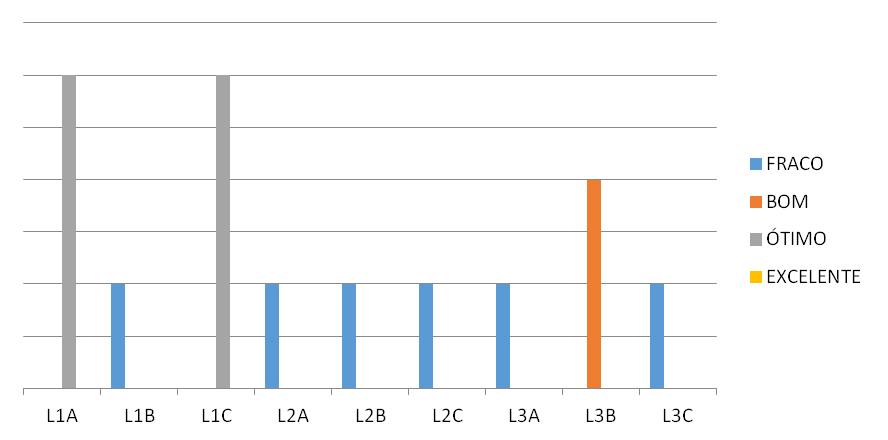
\includegraphics[width=4.625in]{articles/13-educacao-ambiental-n/fig1.png}%
        \label{fig:grafico-freq}%
    \end{figure}%

    Considerando os dados apresentados no gráfico acima se pode concluir que a abordagem da temática ambiental nos livros analisados não se dá de forma gradativa, e isto é preocupante, pois uma vez avançando de série, espera-se que os alunos sejam capazes de desenvolver mais habilidades e competências, tendo em vista estarem finalizando seu processo de formação na educação básica.  


    \section{Considerações finais}

    Na análise dos nove volumes dos livros didáticos de Geografia, para o triênio 2018 a 2020, podemos destacar: A importância dessa análise se dá, sobretudo, à realidade de que o livro didático é uma das principais ferramentas utilizadas para construção do conhecimento dos alunos que estudam na rede pública de ensino do RN.

    A pesquisa realizada ocorreu visando atender a percepção da consonância dos conteúdos integrantes no livro didático da disciplina de geografia nas três séries do ensino médio, com temática ambiental, de suma importância para contribuir para a formação de um cidadão crítico, reflexivo e capaz de criar hábitos ambientais saudáveis de modo que este sujeito em formação possa intervir positivamente na sociedade e contribuir para a transformação da mesma buscando pôr em prática a consciência do ecologicamente correto, socialmente justo e economicamente viável, despertando assim o interesse em desenvolver suas práticas no pensamento do desenvolvimento sustentável.  

    Em relação aos critérios gerais que nortearam a análise dos volumes, foi possível observar que praticamente todos os volumes apresentam conceitos favoráveis (entre Bom e Ótimo), a única exceção foi o critério: “Proposição de experimentos com materiais alternativos de baixo custo”, em que se verificou apenas um conceito B para um dos volumes; os demais foram conceituados como Fraco. Já em relação aos critérios específicos e norteadores de nossa pesquisa, observa-se justamente o contrário: verificou-se em apenas dois volumes conceitos favoráveis: Ótimo e bom. Os demais volumes foram conceituados como fraco (F).  

    Ainda foi possível verificar que os livros de Geografia analisados apresentam um grande abismo e deficiência concernente à presença e o desenvolvimento da temática e questões ambientais que norteiam os conteúdos presentes nos capítulos de suas unidades. Foi constatado que apenas dois volumes abordam de forma bastante satisfatória essa temática, no desenvolvimento de unidades específicas ou permeando outras.  

    Portanto, queremos enfatizar também, baseado em nossa análise que, somente o livro didático de geografia não é responsável por possibilitar meios para a formação de cidadãos no que diz respeito à uma consciência ambiental, ou seja, o mesmo é uma ferramenta que pode dá um auxílio para essa questão.   

    \nocite{BEZERRA2003Temáticas}
    \nocite{LDB1996}
    \nocite{Fundeb2018}
    \nocite{LIMA2006Educação}
    \nocite{GUIALivroDidatico2017}


    \printbibliography[heading=subbibliography,notcategory=fullcited]

    \label{chap:educacao-ambiental-nosend}

\end{refsection}
